% Options for packages loaded elsewhere
\PassOptionsToPackage{unicode}{hyperref}
\PassOptionsToPackage{hyphens}{url}
%
\documentclass[
  12pt,
]{article}
\usepackage[]{mathpazo}
\usepackage{amssymb,amsmath}
\usepackage{ifxetex,ifluatex}
\ifnum 0\ifxetex 1\fi\ifluatex 1\fi=0 % if pdftex
  \usepackage[T1]{fontenc}
  \usepackage[utf8]{inputenc}
  \usepackage{textcomp} % provide euro and other symbols
\else % if luatex or xetex
  \usepackage{unicode-math}
  \defaultfontfeatures{Scale=MatchLowercase}
  \defaultfontfeatures[\rmfamily]{Ligatures=TeX,Scale=1}
\fi
% Use upquote if available, for straight quotes in verbatim environments
\IfFileExists{upquote.sty}{\usepackage{upquote}}{}
\IfFileExists{microtype.sty}{% use microtype if available
  \usepackage[]{microtype}
  \UseMicrotypeSet[protrusion]{basicmath} % disable protrusion for tt fonts
}{}
\makeatletter
\@ifundefined{KOMAClassName}{% if non-KOMA class
  \IfFileExists{parskip.sty}{%
    \usepackage{parskip}
  }{% else
    \setlength{\parindent}{0pt}
    \setlength{\parskip}{6pt plus 2pt minus 1pt}}
}{% if KOMA class
  \KOMAoptions{parskip=half}}
\makeatother
\usepackage{xcolor}
\IfFileExists{xurl.sty}{\usepackage{xurl}}{} % add URL line breaks if available
\IfFileExists{bookmark.sty}{\usepackage{bookmark}}{\usepackage{hyperref}}
\hypersetup{
  pdftitle={CA 3 - Data Analysis},
  hidelinks,
  pdfcreator={LaTeX via pandoc}}
\urlstyle{same} % disable monospaced font for URLs
\usepackage[margin=3cm]{geometry}
\usepackage{color}
\usepackage{fancyvrb}
\newcommand{\VerbBar}{|}
\newcommand{\VERB}{\Verb[commandchars=\\\{\}]}
\DefineVerbatimEnvironment{Highlighting}{Verbatim}{commandchars=\\\{\}}
% Add ',fontsize=\small' for more characters per line
\usepackage{framed}
\definecolor{shadecolor}{RGB}{248,248,248}
\newenvironment{Shaded}{\begin{snugshade}}{\end{snugshade}}
\newcommand{\AlertTok}[1]{\textcolor[rgb]{0.94,0.16,0.16}{#1}}
\newcommand{\AnnotationTok}[1]{\textcolor[rgb]{0.56,0.35,0.01}{\textbf{\textit{#1}}}}
\newcommand{\AttributeTok}[1]{\textcolor[rgb]{0.77,0.63,0.00}{#1}}
\newcommand{\BaseNTok}[1]{\textcolor[rgb]{0.00,0.00,0.81}{#1}}
\newcommand{\BuiltInTok}[1]{#1}
\newcommand{\CharTok}[1]{\textcolor[rgb]{0.31,0.60,0.02}{#1}}
\newcommand{\CommentTok}[1]{\textcolor[rgb]{0.56,0.35,0.01}{\textit{#1}}}
\newcommand{\CommentVarTok}[1]{\textcolor[rgb]{0.56,0.35,0.01}{\textbf{\textit{#1}}}}
\newcommand{\ConstantTok}[1]{\textcolor[rgb]{0.00,0.00,0.00}{#1}}
\newcommand{\ControlFlowTok}[1]{\textcolor[rgb]{0.13,0.29,0.53}{\textbf{#1}}}
\newcommand{\DataTypeTok}[1]{\textcolor[rgb]{0.13,0.29,0.53}{#1}}
\newcommand{\DecValTok}[1]{\textcolor[rgb]{0.00,0.00,0.81}{#1}}
\newcommand{\DocumentationTok}[1]{\textcolor[rgb]{0.56,0.35,0.01}{\textbf{\textit{#1}}}}
\newcommand{\ErrorTok}[1]{\textcolor[rgb]{0.64,0.00,0.00}{\textbf{#1}}}
\newcommand{\ExtensionTok}[1]{#1}
\newcommand{\FloatTok}[1]{\textcolor[rgb]{0.00,0.00,0.81}{#1}}
\newcommand{\FunctionTok}[1]{\textcolor[rgb]{0.00,0.00,0.00}{#1}}
\newcommand{\ImportTok}[1]{#1}
\newcommand{\InformationTok}[1]{\textcolor[rgb]{0.56,0.35,0.01}{\textbf{\textit{#1}}}}
\newcommand{\KeywordTok}[1]{\textcolor[rgb]{0.13,0.29,0.53}{\textbf{#1}}}
\newcommand{\NormalTok}[1]{#1}
\newcommand{\OperatorTok}[1]{\textcolor[rgb]{0.81,0.36,0.00}{\textbf{#1}}}
\newcommand{\OtherTok}[1]{\textcolor[rgb]{0.56,0.35,0.01}{#1}}
\newcommand{\PreprocessorTok}[1]{\textcolor[rgb]{0.56,0.35,0.01}{\textit{#1}}}
\newcommand{\RegionMarkerTok}[1]{#1}
\newcommand{\SpecialCharTok}[1]{\textcolor[rgb]{0.00,0.00,0.00}{#1}}
\newcommand{\SpecialStringTok}[1]{\textcolor[rgb]{0.31,0.60,0.02}{#1}}
\newcommand{\StringTok}[1]{\textcolor[rgb]{0.31,0.60,0.02}{#1}}
\newcommand{\VariableTok}[1]{\textcolor[rgb]{0.00,0.00,0.00}{#1}}
\newcommand{\VerbatimStringTok}[1]{\textcolor[rgb]{0.31,0.60,0.02}{#1}}
\newcommand{\WarningTok}[1]{\textcolor[rgb]{0.56,0.35,0.01}{\textbf{\textit{#1}}}}
\usepackage{longtable,booktabs}
% Correct order of tables after \paragraph or \subparagraph
\usepackage{etoolbox}
\makeatletter
\patchcmd\longtable{\par}{\if@noskipsec\mbox{}\fi\par}{}{}
\makeatother
% Allow footnotes in longtable head/foot
\IfFileExists{footnotehyper.sty}{\usepackage{footnotehyper}}{\usepackage{footnote}}
\makesavenoteenv{longtable}
\usepackage{graphicx}
\makeatletter
\def\maxwidth{\ifdim\Gin@nat@width>\linewidth\linewidth\else\Gin@nat@width\fi}
\def\maxheight{\ifdim\Gin@nat@height>\textheight\textheight\else\Gin@nat@height\fi}
\makeatother
% Scale images if necessary, so that they will not overflow the page
% margins by default, and it is still possible to overwrite the defaults
% using explicit options in \includegraphics[width, height, ...]{}
\setkeys{Gin}{width=\maxwidth,height=\maxheight,keepaspectratio}
% Set default figure placement to htbp
\makeatletter
\def\fps@figure{htbp}
\makeatother
\setlength{\emergencystretch}{3em} % prevent overfull lines
\providecommand{\tightlist}{%
  \setlength{\itemsep}{0pt}\setlength{\parskip}{0pt}}
\setcounter{secnumdepth}{-\maxdimen} % remove section numbering
\usepackage{titling}
\usepackage{pdfpages}
\usepackage{atbegshi}% http://ctan.org/pkg/atbegshi
\usepackage{threeparttable}
\usepackage{multirow}
\usepackage{booktabs}
\usepackage{float}
\usepackage{ragged2e}

\AtBeginDocument{\AtBeginShipoutNext{\AtBeginShipoutDiscard}}
\pretitle{%
  \begin{center}
  \LARGE
  
\includepdf[pages=-]{cover_sheet.pdf}
}
\posttitle{\end{center}}
\usepackage{booktabs}
\usepackage{longtable}
\usepackage{array}
\usepackage{multirow}
\usepackage{wrapfig}
\usepackage{float}
\usepackage{colortbl}
\usepackage{pdflscape}
\usepackage{tabu}
\usepackage{threeparttable}
\usepackage{threeparttablex}
\usepackage[normalem]{ulem}
\usepackage{makecell}
\usepackage{xcolor}
\newlength{\cslhangindent}
\setlength{\cslhangindent}{1.5em}
\newenvironment{cslreferences}%
  {\setlength{\parindent}{0pt}%
  \everypar{\setlength{\hangindent}{\cslhangindent}}\ignorespaces}%
  {\par}

\title{CA 3 - Data Analysis}
\usepackage{etoolbox}
\makeatletter
\providecommand{\subtitle}[1]{% add subtitle to \maketitle
  \apptocmd{\@title}{\par {\large #1 \par}}{}{}
}
\makeatother
\subtitle{Health in Ireland}
\author{}
\date{\vspace{-2.5em}}

\begin{document}
\maketitle

\setcounter{page}{1}
\renewcommand{\arraystretch}{1.5}
\renewcommand{\footnotesize}{\small \justify}

\begingroup
\setlength{\tabcolsep}{15pt} 
\renewcommand{\arraystretch}{1.5} 
  \begin{tabular}[]{@{}ll@{}}
    \bf Title:      & Trends in Irish hospital waiting list figures \\
    \bf Author:     & Danny Regan \\
    \bf Supervisor: & Dr James Connolly \\
    \bf Degree:     & MSc in Big Data Analytics \\
    \bf Module:     & Data Science \\
    \bf Github:     & \url{https://github.com/ancodia/hospital_waiting_lists}
  \end{tabular}
\endgroup

\hypertarget{abstract}{%
\section{Abstract}\label{abstract}}

Waiting lists for procedures in Irish public hospitals are some of the longest in Europe. The National Treatment Purchase Fund (NTPF) is the organisation responsible with collecting data about patients on these lists. This project uses the NTPF data to examine the question of what trends are present within it and determine what similarities or differences exist between those trends. To answer this research question the Mann-Kendall and Sen's slope statistical tests are applied to the data to verify if trends exist and the magnitude of those trends respectively.

The results returned from applying these tests show that, with the exception of the group containing all patents waiting under a year for a procedure, increasing trends are the norm. This result confirms that serious issues with the operation of the Irish health system need to be addressed and further research could build on what is presented here to investigate the problems in finer detail.

\newpage

\hypertarget{introduction}{%
\section{Introduction}\label{introduction}}

The volume of patients waiting for hospital procedures and the length of these waits constitute a major shortfall in the Irish public healthcare system. According to the most recent Euro Health Consumer Index (Health Consumer Powerhouse \protect\hyperlink{ref-health_consumer_powerhouse_euro_2018}{2018}, p.15), Ireland has the longest waiting times in Europe despite having one of the greatest levels of expenditure on health (OECD and European Union \protect\hyperlink{ref-oecd_health_2018}{2018}, p.133).

The National Treatment Purchase Fund (NTPF) is the organisation assigned the task by the Irish government of collecting, collating and validating data about individuals who are waiting for treatment in public hospitals. This is the source of data for the current project.

A description of the data and steps taken to clean it are the feature of the next section. This data description section also includes justification for choices of statistical methods to aid in answering the research question displayed below. The sections that follow this cover the hypothesis testing to be carried on the waiting list data and reporting and discussion of results obtained from the analysis undertaken.

\hypertarget{research-question}{%
\subsubsection{Research Question}\label{research-question}}

The NTPF waiting list data will be used in this project to answer the following research question:

\begin{quote}
What differences, if any, exist among trends found in Irish hospital group waiting list figures from recent years?
\end{quote}

\hypertarget{data-description}{%
\section{Data Description}\label{data-description}}

The data for this project comes from that collected by NTPF for outpatient (OP)\footnote{\url{https://data.ehealthireland.ie/dataset/op-waiting-list-by-group-hospital}}, inpatient/day case (IPDC)\footnote{\url{https://data.ehealthireland.ie/dataset/ipdc-waiting-list-by-group-hospital}} and GI endoscopy (IPDC GI)\footnote{\url{https://data.ehealthireland.ie/dataset/ipdc-gi-endoscopy-by-group-hospital}} waiting list numbers for all public hospitals across Ireland. The data that is being considered is monthly totals from January 2014 to December 2019. This section describes how the data was prepared for analysis and which statistical methods were chosen to assist in answering the research question.

\begin{table}

\caption{\label{tab:waiting-list-counts}Waiting list counts.}
\centering
\begin{tabular}[t]{lr}
\toprule
Waiting list & Patient count\\
\midrule
OP: & 481643\\
IPDC: & 294977\\
IPDC GI: & 36978\\
\hline
Overall: & 813598\\
\bottomrule
\end{tabular}
\end{table}

\newpage

\hypertarget{data-cleaning}{%
\subsection{Data Cleaning}\label{data-cleaning}}

R code referenced in this section is found in \texttt{data\_prep/data\_transformation.R}.

\hypertarget{amalgamating-source-data}{%
\subsubsection{Amalgamating source data}\label{amalgamating-source-data}}

The first step necessary is to combine all data into a single dataset. This is accomplished by initially combining all csv files for each waiting list category with the \texttt{combine\_csv\_data()} function in \texttt{helpers/data\_prep\_helper.R} which uses the \texttt{vroom} package. Then the 3 resulting tibbles are combined with \texttt{dplyr::bindrows}. The row counts for the individual and combined datasets can be seen in Table \ref{tab:waiting-list-counts} while Table \ref{tab:sample-rows} shows a sample of rows from the overall data. The format of archive dates varies between Y-m-d and d/m/Y so the \texttt{convert\_dates()} function that makes use of \texttt{libridate::parse\_date\_time} to convert all to a single datetime format was added to the \texttt{data\_prep\_helper.R} helper file.

\begin{table}[!h]

\caption{\label{tab:sample-rows}Random sample of rows from the combined data.}
\centering
\resizebox{\linewidth}{!}{
\begin{tabular}[t]{llllllllllr}
\toprule
\rotatebox{45}{Archive\_Date} & \rotatebox{45}{Hospital\_Group} & \rotatebox{45}{Hospital\_HIPE} & \rotatebox{45}{Hospital\_Name} & \rotatebox{45}{Speciality\_HIPE} & \rotatebox{45}{Speciality\_Name} & \rotatebox{45}{Case\_Type} & \rotatebox{45}{Adult\_Child} & \rotatebox{45}{Age\_Profile} & \rotatebox{45}{Time\_Bands} & \rotatebox{45}{Total}\\
\midrule
2015-02-26 & Children's Hospital Group & 0941 & Our Lady's Children's Hospital Crumlin & 2600 & General Surgery & NA & Child & 0-15 & 15-18 Months & 36\\
2014-05-30 & University of Limerick Hospital Group & 0305 & Ennis Hospital & 2600 & General Surgery & NA & Adult & 65+ & 6-9 Months & 43\\
2017-05-31 & Children's Hospital Group & 0941 & Our Lady's Children's Hospital Crumlin & 1905 & Paed Endocrinology & NA & Child & 0-15 & 6-9 Months & 11\\
2015-03-26 & Ireland East Hospital Group & 0908 & Mater Misericordiae University Hospital & 7000 & Dental Surgery & Day Case & Adult & 16-64 & 3-6 Months & 2\\
2016-05-31 & RCSI  Hospitals Group & 0400 & Louth County Hospital & 2600 & General Surgery & NA & Adult & 65+ & 3-6 Months & 7\\
\addlinespace
30/01/2020 & Ireland East Hospital Group & 0101 & St. Columcille's Hospital & 2100 & Psychiatry & NA & Adult & 65+ & 6-9 Months & 2\\
2016-08-31 & Saolta University Health Care Group & 0500 & Letterkenny General Hospital & 0100 & Cardiology & Day Case & Adult & 65+ & 0-3 Months & 22\\
2014-10-31 & University of Limerick Hospital Group & 0304 & Nenagh Hospital & 2604 & Vascular Surgery & NA & Child & 0-15 & 3-6 Months & 1\\
2015-07-30 & Dublin Midlands Hospital Group & 0102 & Naas General Hospital & 5000 & General Medicine & Day Case & Adult & 16-64 & 6-9 Months & 50\\
28/02/2018 & Saolta University Health Care Group & 803 & Roscommon University Hospital & 2600 & General Surgery & Day Case & Adult & 65+ & 0-3 Months & 12\\
\addlinespace
20/12/2018 & South/South West Hospital Group & 913 & Mercy University Hospital & 8003 & Pain Relief & NA & Adult & 16-64 & 3-6 Months & 77\\
2016-09-29 & Ireland East Hospital Group & 0601 & St. Luke's General Hospital Kilkenny & 1503 & Gynaecology & NA & Adult & 16-64 & 12-15 Months & 57\\
31/05/2018 & Ireland East Hospital Group & 202 & Midland Regional Hospital Mullingar & 1700 & Ophthalmology & NA & Child & 0-15 & 9-12 Months & 1\\
2014-09-26 & Ireland East Hospital Group & 0908 & Mater Misericordiae University Hospital & 0300 & Dermatology & NA & Adult & 65+ & 6-9 Months & 100\\
25/04/2019 & Ireland East Hospital Group & 0908 & Mater Misericordiae University Hospital & 0700 & Gastro-Enterology & NA & Adult & 65+ & 9-12 Months & 12\\
\bottomrule
\end{tabular}}
\end{table}

\begin{figure}

{\centering 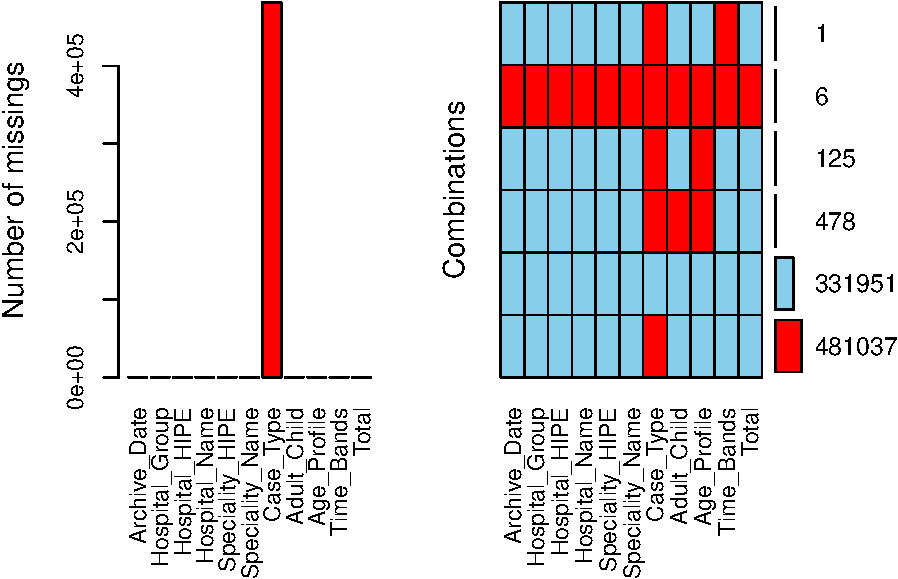
\includegraphics{data_science_ca3_files/figure-latex/missing-values-1} 

}

\caption{Missing values.}\label{fig:missing-values}
\end{figure}

\hypertarget{dealing-with-missing-values}{%
\subsubsection{Dealing with missing values}\label{dealing-with-missing-values}}

Missing values from the combined data are displayed in Figure \ref{fig:missing-values}. The following steps were taken to handle these.

The missing case types are expected for all outpatient records because that column does not exist in the source csv so those are assigned a value of ``Outpatient'':
\small

\begin{Shaded}
\begin{Highlighting}[]
\NormalTok{all\_waiting\_lists}\OperatorTok{$}\NormalTok{Case\_Type[}\KeywordTok{is.na}\NormalTok{(all\_waiting\_lists}\OperatorTok{$}\NormalTok{Case\_Type)] \textless{}{-}}\StringTok{ "Outpatient"} 
\end{Highlighting}
\end{Shaded}

\normalsize

There are 6 blank records introduced from the source datasets explaining the missing values for Archive\_Date, Hospital\_Group, Hospital\_HIPE, Hospital\_Name, Speciality\_HIPE, Speciality\_Name, Time\_Bands and Total so these are dropped:

\begin{Shaded}
\begin{Highlighting}[]
\NormalTok{all\_waiting\_lists \textless{}{-}}\StringTok{ }\KeywordTok{subset}\NormalTok{(all\_waiting\_lists, }
                            \OperatorTok{!}\KeywordTok{is.na}\NormalTok{(all\_waiting\_lists}\OperatorTok{$}\NormalTok{Hospital\_Name))}
\KeywordTok{nrow}\NormalTok{(all\_waiting\_lists)}
\end{Highlighting}
\end{Shaded}

\begin{verbatim}
## [1] 813592
\end{verbatim}

The 1 remaining row with a missing Time\_Bands value is also removed because time band is vital for the analysis that follows:
\small

\begin{Shaded}
\begin{Highlighting}[]
\KeywordTok{nrow}\NormalTok{(all\_waiting\_lists)}
\end{Highlighting}
\end{Shaded}

\begin{verbatim}
## [1] 813592
\end{verbatim}

\begin{Shaded}
\begin{Highlighting}[]
\NormalTok{all\_waiting\_lists \textless{}{-}}\StringTok{ }\NormalTok{all\_waiting\_lists[}\OperatorTok{!}\KeywordTok{is.na}\NormalTok{(all\_waiting\_lists}\OperatorTok{$}\NormalTok{Time\_Bands),]}
\KeywordTok{nrow}\NormalTok{(all\_waiting\_lists)}
\end{Highlighting}
\end{Shaded}

\begin{verbatim}
## [1] 813591
\end{verbatim}

\normalsize

All other missing values are deemed irrelevant for the current project, so no action is taken.

\hypertarget{time-band-formatting}{%
\subsubsection{Time band formatting}\label{time-band-formatting}}

The time bands variable originally had variations of the same values:
\small

\begin{Shaded}
\begin{Highlighting}[]
\KeywordTok{unique}\NormalTok{(all\_waiting\_lists[, }\KeywordTok{c}\NormalTok{(}\StringTok{"Time\_Bands"}\NormalTok{)])}
\end{Highlighting}
\end{Shaded}

\begin{verbatim}
## # A tibble: 12 x 1
##    Time_Bands    
##    <chr>         
##  1 "0-3 Months"  
##  2 "3-6 Months"  
##  3 "6-9 Months"  
##  4 "9-12 Months" 
##  5 "15-18 Months"
##  6 "18+ Months"  
##  7 "12-15 Months"
##  8 "18 Months +" 
##  9 " 0-3 Months" 
## 10 " 9-12 Months"
## 11 " 3-6 Months" 
## 12 " 6-9 Months"
\end{verbatim}

\normalsize

To rectify these differences whitespace was removed from all and the format for ``18+ months'' was standardised:

\begin{Shaded}
\begin{Highlighting}[]
\NormalTok{all\_waiting\_lists}\OperatorTok{$}\NormalTok{Time\_Bands \textless{}{-}}\StringTok{ }\KeywordTok{as.character}\NormalTok{(all\_waiting\_lists}\OperatorTok{$}\NormalTok{Time\_Bands)}
\NormalTok{all\_waiting\_lists}\OperatorTok{$}\NormalTok{Time\_Bands \textless{}{-}}\StringTok{ }\KeywordTok{trimws}\NormalTok{(all\_waiting\_lists}\OperatorTok{$}\NormalTok{Time\_Bands)}
\NormalTok{all\_waiting\_lists}\OperatorTok{$}\NormalTok{Time\_Bands[}
\NormalTok{  all\_waiting\_lists}\OperatorTok{$}\NormalTok{Time\_Bands }\OperatorTok{==}\StringTok{ "18 Months +"}\NormalTok{] \textless{}{-}}\StringTok{ "18+ Months"}
\end{Highlighting}
\end{Shaded}

With the result looking like so:
\small

\begin{Shaded}
\begin{Highlighting}[]
\KeywordTok{unique}\NormalTok{(all\_waiting\_lists[, }\KeywordTok{c}\NormalTok{(}\StringTok{"Time\_Bands"}\NormalTok{)])}
\end{Highlighting}
\end{Shaded}

\begin{verbatim}
## # A tibble: 7 x 1
##   Time_Bands  
##   <chr>       
## 1 0-3 Months  
## 2 3-6 Months  
## 3 6-9 Months  
## 4 9-12 Months 
## 5 15-18 Months
## 6 18+ Months  
## 7 12-15 Months
\end{verbatim}

\normalsize

To perform the analysis for answering the defined research question it was decided to reduce time band to 2 groupings, less than a year and greater than a year waiting:
\small

\begin{Shaded}
\begin{Highlighting}[]
\KeywordTok{unique}\NormalTok{(all\_waiting\_lists[, }\KeywordTok{c}\NormalTok{(}\StringTok{"Time\_Bands"}\NormalTok{)])}
\end{Highlighting}
\end{Shaded}

\begin{verbatim}
## # A tibble: 2 x 1
##   Time_Bands
##   <fct>     
## 1 < 1 Year  
## 2 > 1 Year
\end{verbatim}

\normalsize

\hypertarget{removal-of-unnecessary-variables}{%
\subsubsection{Removal of unnecessary variables}\label{removal-of-unnecessary-variables}}

Columns that aren't necessary for this project were removed from the dataset. The analysis will examine trends by using the 7 hospital groups and the 2 newly created waiting list time band so only the Archive\_Date, Hospital\_Group, Time\_Bands and Total variables are kept.

Structure before removal:
\small

\begin{Shaded}
\begin{Highlighting}[]
\KeywordTok{str}\NormalTok{(all\_waiting\_lists, }\DataTypeTok{width =} \DecValTok{70}\NormalTok{, }\DataTypeTok{strict.width =} \StringTok{"cut"}\NormalTok{)}
\end{Highlighting}
\end{Shaded}

\begin{verbatim}
## tibble [813,591 x 11] (S3: tbl_df/tbl/data.frame)
##  $ Archive_Date   : chr [1:813591] "31/10/2019" "31/10/2019" "31/10"..
##  $ Hospital_Group : chr [1:813591] "Children's Health Ireland" "Chi"..
##  $ Hospital_HIPE  : chr [1:813591] "0000" "0000" "0000" "0000" ...
##  $ Hospital_Name  : chr [1:813591] "Children's Health Ireland" "Chi"..
##  $ Speciality_HIPE: chr [1:813591] "0000" "0601" "0601" "0601" ...
##  $ Speciality_Name: chr [1:813591] "Small Volume Specialities" "Pae"..
##  $ Case_Type      : chr [1:813591] "Day Case" "Day Case" "Day Case""..
##  $ Adult_Child    : chr [1:813591] "Child" "Child" "Child" "Child" ...
##  $ Age_Profile    : chr [1:813591] "0-15" "0-15" "0-15" "0-15" ...
##  $ Time_Bands     : Factor w/ 2 levels "< 1 Year","> 1 Year": 1 1 1 ..
##  $ Total          : num [1:813591] 1 71 26 20 1 2 4 4 2 136 ...
\end{verbatim}

\normalsize

After removal:
\small

\begin{Shaded}
\begin{Highlighting}[]
\KeywordTok{str}\NormalTok{(all\_waiting\_lists, }\DataTypeTok{width =} \DecValTok{70}\NormalTok{, }\DataTypeTok{strict.width =} \StringTok{"cut"}\NormalTok{)}
\end{Highlighting}
\end{Shaded}

\begin{verbatim}
## tibble [813,591 x 4] (S3: tbl_df/tbl/data.frame)
##  $ Archive_Date  : chr [1:813591] "31/10/2019" "31/10/2019" "31/10/"..
##  $ Hospital_Group: chr [1:813591] "Children's Health Ireland" "Chil"..
##  $ Time_Bands    : Factor w/ 2 levels "< 1 Year","> 1 Year": 1 1 1 1..
##  $ Total         : num [1:813591] 1 71 26 20 1 2 4 4 2 136 ...
\end{verbatim}

\normalsize

\hypertarget{final-clean-up}{%
\subsubsection{Final clean up}\label{final-clean-up}}

The final steps in the data cleaning process involved abbreviating the hospital group names and excluding records from 2020 in the data as these only consist of January figures. The name abbreviation was done to accommodate displaying the names in charts that follow.

Note: The Children's Hospital Group was renamed to Children's Health Ireland in 2018 so these are classed as a single group.

Original hospital group names:
\small

\begin{Shaded}
\begin{Highlighting}[]
\KeywordTok{unique}\NormalTok{(all\_waiting\_lists[, }\KeywordTok{c}\NormalTok{(}\StringTok{"Hospital\_Group"}\NormalTok{)])}
\end{Highlighting}
\end{Shaded}

\begin{verbatim}
## # A tibble: 8 x 1
##   Hospital_Group                       
##   <chr>                                
## 1 Children's Health Ireland            
## 2 Dublin Midlands Hospital Group       
## 3 Ireland East Hospital Group          
## 4 RCSI  Hospitals Group                
## 5 Saolta University Health Care Group  
## 6 South/South West Hospital Group      
## 7 University of Limerick Hospital Group
## 8 Children's Hospital Group
\end{verbatim}

\normalsize

Abbreviated hospital group names:
\small

\begin{Shaded}
\begin{Highlighting}[]
\KeywordTok{unique}\NormalTok{(all\_waiting\_lists[, }\KeywordTok{c}\NormalTok{(}\StringTok{"Hospital\_Group"}\NormalTok{)])}
\end{Highlighting}
\end{Shaded}

\begin{verbatim}
## [1] "CHI"              "Dublin Midlands"  "Ireland East"     "RCSI"            
## [5] "Saolta"           "South/South West" "UL"
\end{verbatim}

\normalsize

A csv file named \texttt{combined\_waiting\_lists.csv} containing the processed data is found in the \texttt{data\_prep} directory.

\newpage

\hypertarget{choice-of-statistical-methods}{%
\subsection{Choice of Statistical Methods}\label{choice-of-statistical-methods}}

\label{sec:stats-methods}
Figure \ref{fig:totals-img} shows all waiting lists plotted as a bar chart to give a general view of how the data has changed over time. The trend here appears to be generally ever growing numbers of patients waiting more than a year for procedures while those waiting less than a year saw a steady increase from 2014 to 2017 and a stabling thereafter.

\begin{figure}[h]

{\centering 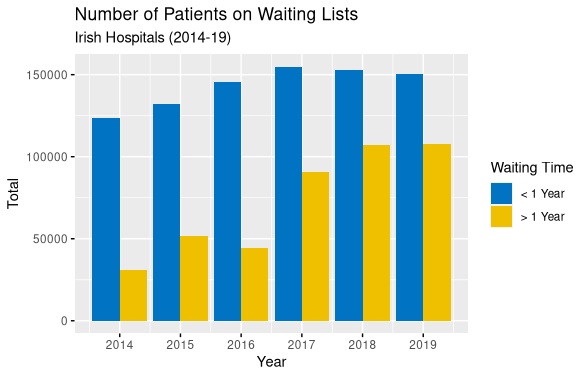
\includegraphics[width=0.7\linewidth,height=0.7\textheight]{/home/danny/MEGA/College/msc_data_analytics/data_science/ca3/hospital_waiting_lists/documentation/images/waiting_list_totals} 

}

\caption{Totals waiting list numbers by year.}\label{fig:totals-img}
\end{figure}

To help decide what type of statistical methods are suitable for use on this data, density plots for each hospital group were generated, see Figure \ref{fig:densities-img}. All groups have skewed distributions meaning some type of non-parametric methods must be used.

\begin{figure}

{\centering 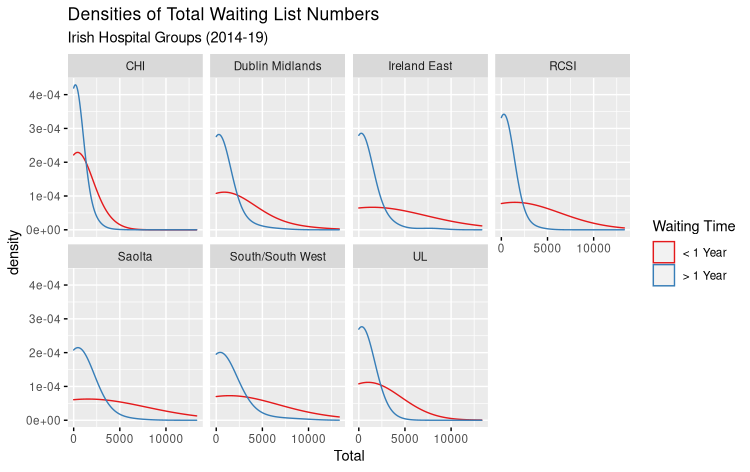
\includegraphics{/home/danny/MEGA/College/msc_data_analytics/data_science/ca3/hospital_waiting_lists/documentation/images/densities} 

}

\caption{Density plot for each Irish hospital group.}\label{fig:densities-img}
\end{figure}

Based on the data being time series in nature and not normally distributed the chosen statistical tests to answer the research question are the Mann-Kendall test to determine if monotonic trends are present and the Sen's slope test to check the magnitude of trends, if they exist.

\newpage

\hypertarget{hypothesis-testing}{%
\section{Hypothesis Testing}\label{hypothesis-testing}}

The hypothesis being tested on the waiting list time series data with the Mann-Kendall test is as follows:

\(H_0\): No monotonic trend exists

\(H_1\): Monotonic trend exists

Code relating to the testing of this hypothesis is found in the \texttt{time\_series\_analysis} function in \texttt{helpers/descriptive\_statistics\_helper.R}.

The Mann-Kendall test is performed with \texttt{Kendall::MannKendall} which returns a score and a p-value, 2-sided in this case. For this test, a confidence interval of 95\% is used meaning a p-value of less than 0.05 is necessary to reject the null hypothesis

The Sen's slope test is performed to determine the magnitude of the monotonic trend, if present. The \texttt{trend::sens.slope} function provides this test.

The overall data is split into individual datasets for each hospital group in order to facilitate testing. The next section discusses the results obtained by using this combination of tests.

\newpage

\hypertarget{results}{%
\section{Results}\label{results}}

Results from performing the Mann-Kendall and Sen's Slope tests on the overall data and each of the individual hospital groups can be seen in Table \ref{tab:timeseries}. Code relevant to this section is found in \texttt{data\_analysis/analyse\_prepared\_waiting\_list\_data.}. Discussion about the results is featured below and plots of the decomposition of each time series group can be found in the \hyperref[sec:appendix]{Appendix}.

\begin{table*}[!htbp]
    \centering
    \caption{Time series analysis results}\label{tab:timeseries}
    \begin{threeparttable}
    \begin{tabular}{ll|lll|ll}
        \toprule
          & & \multicolumn{3}{c}{\bfseries Mann-Kendall} & \multicolumn{2}{c}{\bfseries Sen's Slope} \\ \hline
          
            & & \bfseries Score & \bfseries p-value & \bfseries Result & \bfseries Slope & \bfseries p-value  \\
            \midrule
            \multirow{2}{*}{All}      & < 1 Yr (\hyperref[fig:ts-overall-lt1yr]{Fig. 4}) 
                                      & 232 & 0.26146 & No Trend & 58.38 & 0.2615 \\
                                      
                                      & > 1 Yr (\hyperref[fig:ts-overall-gt1yr]{Fig. 5}) 
                                      & 1084 & < 0.0001 & Increasing & 77.89 & < 0.0001 \\ \hline
                                      
        \multirow{2}{*}{CHI}      & < 1 Yr (\hyperref[fig:ts-chi-lt1yr]{Fig. 6}) 
                                  & 1508 & < 0.0001 & Increasing & 126.61 & < 0.0001 \\
                                  
                                      & > 1 Yr (\hyperref[fig:ts-chi-gt1yr]{Fig. 7})
                                      & 2238 & < 0.0001 & Increasing & 312.91 & < 0.0001 \\ \hline
                                      
        \multirow{2}{*}{Dub. Mid.} & < 1 Yr (\hyperref[fig:ts-dm-lt1yr]{Fig. 8}) 
                                  & 1966 & < 0.0001 & Increasing & 158.69 & < 0.0001 \\
                                  
                                      & > 1 Yr (\hyperref[fig:ts-dm-gt1yr]{Fig. 9})
                                      & 2098 & < 0.0001 & Increasing & 415.79 & < 0.0001 \\ \hline
                                      
        \multirow{2}{*}{Ire. East} & < 1 Yr (\hyperref[fig:ts-ie-lt1yr]{Fig. 10}) 
                                  & 2180 & < 0.0001 & Increasing & 158.69 & < 0.0001 \\
                                  
                                      & > 1 Yr (\hyperref[fig:ts-ie-gt1yr]{Fig. 11})
                                      & 2314 & < 0.0001 & Increasing & 515.56 & < 0.0001 \\ \hline
                           
        \multirow{2}{*}{RCSI} & < 1 Yr (\hyperref[fig:ts-rcsi-lt1yr]{Fig. 12}) 
                                  & 884 & < 0.0001 & Increasing & 65.95 & < 0.0001 \\
                                  
                                      & > 1 Yr (\hyperref[fig:ts-rcsi-gt1yr]{Fig. 13})
                                      & 648 & 0.0016596 & Increasing & 103.62 & 0.00166 \\ \hline
                                      
        \multirow{2}{*}{Saolta} & < 1 Yr (\hyperref[fig:ts-saolta-lt1yr]{Fig. 14}) 
                                  & 2042 & < 0.0001 & Increasing & 235.46 & < 0.0001 \\
                                  
                                      & > 1 Yr (\hyperref[fig:ts-saolta-gt1yr]{Fig. 15})
                                      & 2078 & < 0.0001 & Increasing & 382.67 & < 0.0001 \\ \hline
                                      
        \multirow{2}{*}{UL} & < 1 Yr (\hyperref[fig:ts-ul-lt1yr]{Fig. 16}) 
                                  & 2152 & < 0.0001 & Increasing & 171.69 & < 0.0001 \\
                                  
                                      & > 1 Yr (\hyperref[fig:ts-ul-gt1yr]{Fig. 17})
                                      & 2404 & < 0.0001 & Increasing & 284.23 & < 0.0001 \\ \hline
                                     
        \multirow{2}{*}{South/SW} & < 1 Yr (\hyperref[fig:ts-ssw-lt1yr]{Fig. 18}) 
                                  & 931 & < 0.0001 & Increasing & 134.20 & < 0.0001 \\
                                  
                                      & > 1 Yr (\hyperref[fig:ts-ssw-gt1yr]{Fig. 19})
                                      & 2110 & < 0.0001 & Increasing & 521.42 & < 0.0001 \\ \hline
        \bottomrule
    \end{tabular}
    \begin{tablenotes}
      \small
      \item Note: p-values have been rounded for readability when very small values were found. For example, the actual p-value for MK test on all waiting list < 1 year is 1.1921e-07, displayed here as < 0.0001. Sen's slope values have also been rounded (to 2 decimal places). 
    \end{tablenotes}
    \end{threeparttable}
\end{table*}

\newpage

In general, increasing monotonic trends were the norm found when applying the stated statistical techniques to the groups of waiting lists. The result for the group containing all patients waiting less than a year is the only one that does not conform to this generality. Its Mann-Kendall score (232) indicates it is a mainly increasing time series, although from the corresponding graph (\hyperref[fig:ts-overall-lt1yr]{Figure 4}) it is clear there is no consistent trend present. With the exception of the greater than a year waiting group for RCSI, all other p-values for the Mann-Kendall test are extremely low. Numbers for that RCSI group have seen a steady decline since 2018 (\hyperref[fig:ts-rcsi-gt1yr]{Figure 13}) thus explaining the reduced confidence level of the test.

Using the Sen's slope test gives an indication of how great the magnitude of a given trend is which provides a useful means for comparing similar trends. The patients waiting more than a year for procedures in South/South West Hospital group (\hyperref[fig:ts-ssw-gt1yr]{Figure 19}) returned the highest slope value. This signifies that the increasing trend observed has the largest average growth rate of the groups studied.

\hypertarget{conclusions}{%
\section{Conclusions}\label{conclusions}}

The stated aim of this project was to examine trends in waiting list data for Irish public hospitals and determine if any significant differences are observable. To enable this work, data collected by the NTPF for each category of waiting was gathered and processed. The processing involved combining csv files containing monthly waiting list figures going back as far as January 2014. The source data contains records for each list speciality, hospital and trimonthly time band slots. Categorisation was performed on the overall dataset, focused on dividing it into hospital groupings and waiting time bands of less than or greater than a year to facilitate the analysis section of this research.

To answer the project's research question, the Mann-Kendall and Sen's slope statistical trend tests were applied to each of the groups created from the waiting list data. The general result found from these tests was that all of the observed waiting list groups feature an increasing monotonic trend, except the combination of all patients waiting for less than a year. The group containing patient numbers waiting for longer than a year with South/South West Hospital group hospitals returned the highest magnitude from the use of the Sen's slope test. These tests confirmed the assumption made when the total figures were examined initially that increasing trends are the norm (see \hyperref[sec:stats-methods]{Choice of Statistical Methods})

Further work on this research that was neglected from the scope of this project due to time constraints is to examine how trends differ between individual procedure waiting lists. Knowing where the main problem areas exist with evidence confirmed with statistical methods could aid the Department of Health in distributing resources to areas most in need.

\hypertarget{references}{%
\section{References}\label{references}}

\hypertarget{refs}{}
\begin{cslreferences}
\leavevmode\hypertarget{ref-health_consumer_powerhouse_euro_2018}{}%
Health Consumer Powerhouse (2018) \emph{Euro Health Consumer Index 2018} {[}online{]}, Health Consumer Powerhouse, available: \url{https://healthpowerhouse.com/media/EHCI-2018/EHCI-2018-report.pdf} {[}accessed 17 Mar 2020{]}.

\leavevmode\hypertarget{ref-oecd_health_2018}{}%
OECD, European Union (2018) \emph{Health at a Glance: Europe 2018: State of Health in the EU Cycle} {[}online{]}, Health at a glance: Europe, OECD, available: \url{https://www.oecd-ilibrary.org/social-issues-migration-health/health-at-a-glance-europe-2018_health_glance_eur-2018-en} {[}accessed 18 Mar 2020{]}.
\end{cslreferences}

\newpage

\hypertarget{appendix}{%
\section{Appendix}\label{appendix}}

\label{sec:appendix}
\appendix

\hypertarget{decomposed-time-series-plots}{%
\subsubsection{Decomposed Time Series Plots}\label{decomposed-time-series-plots}}

The following plots show the seasonal and trend decomposition for each of the waiting list groups using Loess (locally estimated scatterplot smoothing). This was achieved by calling the \texttt{stats::stl} function on each time series when plotting.

\begin{figure}

{\centering 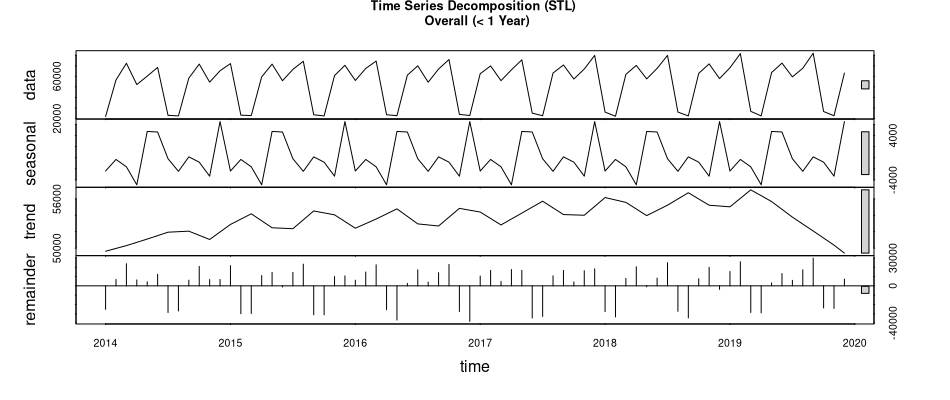
\includegraphics[width=0.7\linewidth]{/home/danny/MEGA/College/msc_data_analytics/data_science/ca3/hospital_waiting_lists/documentation/images/ts_overall_lt1yr} 

}

\caption{Time Series Decomposition - Overall patient numbers waiting less than a year.}\label{fig:ts-overall-lt1yr}
\end{figure}

\begin{figure}

{\centering 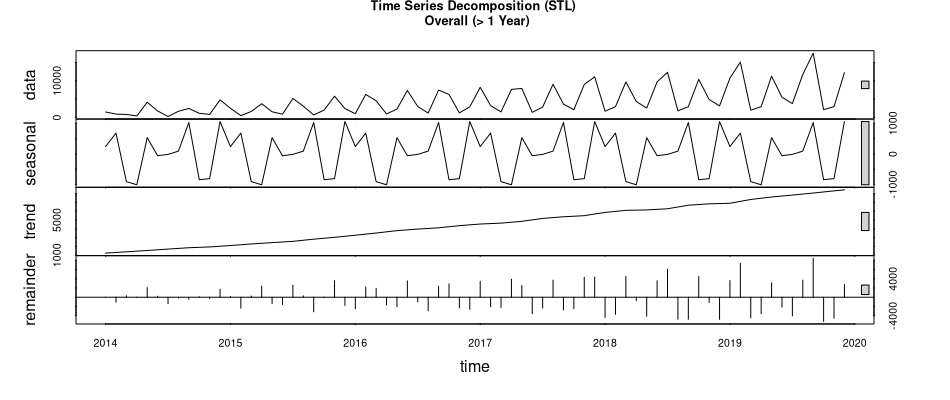
\includegraphics[width=0.7\linewidth]{/home/danny/MEGA/College/msc_data_analytics/data_science/ca3/hospital_waiting_lists/documentation/images/ts_overall_gt1yr} 

}

\caption{Time Series Decomposition - Overall patient numbers waiting more than a year.}\label{fig:ts-overall-gt1yr}
\end{figure}

\begin{figure}

{\centering 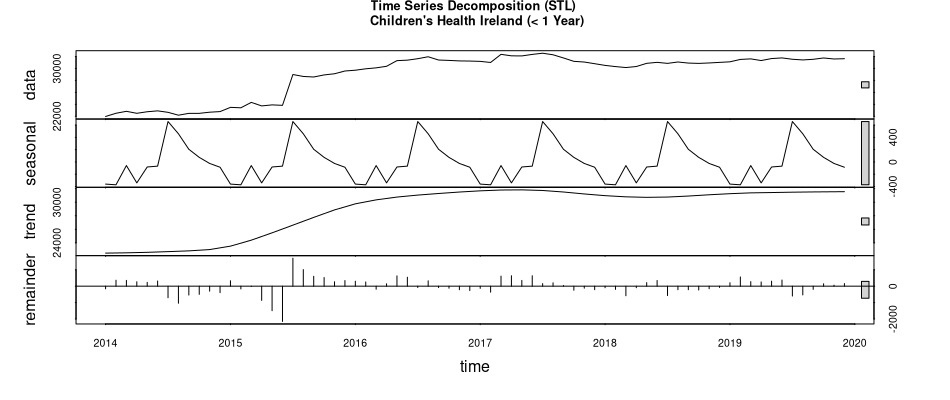
\includegraphics[width=0.7\linewidth]{/home/danny/MEGA/College/msc_data_analytics/data_science/ca3/hospital_waiting_lists/documentation/images/ts_chi_lt1yr} 

}

\caption{Time Series Decomposition - Children's Health Ireland patient numbers waiting less than a year.}\label{fig:ts-chi-lt1yr}
\end{figure}

\begin{figure}

{\centering 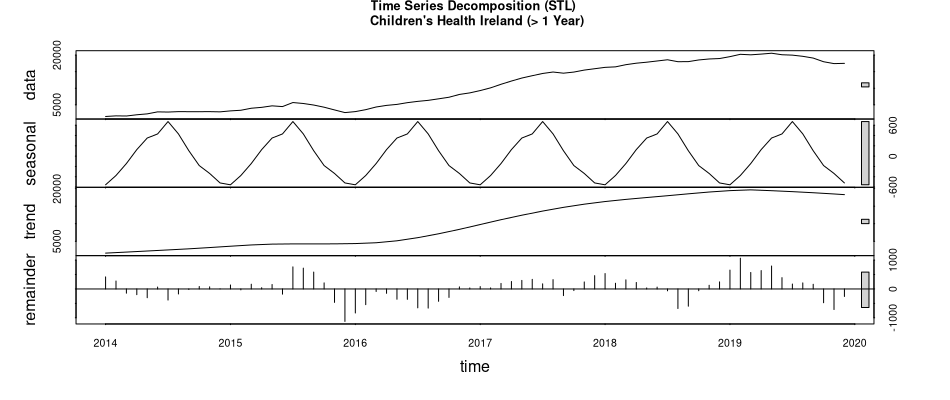
\includegraphics[width=0.7\linewidth]{/home/danny/MEGA/College/msc_data_analytics/data_science/ca3/hospital_waiting_lists/documentation/images/ts_chi_gt1yr} 

}

\caption{Time Series Decomposition - Children's Health Ireland patient numbers waiting more than a year.}\label{fig:ts-chi-gt1yr}
\end{figure}

\begin{figure}

{\centering 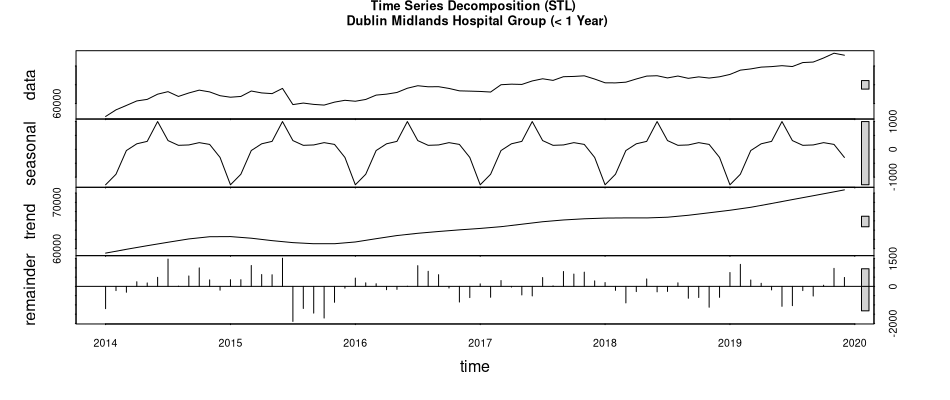
\includegraphics[width=0.7\linewidth]{/home/danny/MEGA/College/msc_data_analytics/data_science/ca3/hospital_waiting_lists/documentation/images/ts_dm_lt1yr} 

}

\caption{Time Series Decomposition - Dublin Midland Hospital Group patient numbers waiting less than a year.}\label{fig:ts-dm-lt1yr}
\end{figure}

\begin{figure}

{\centering 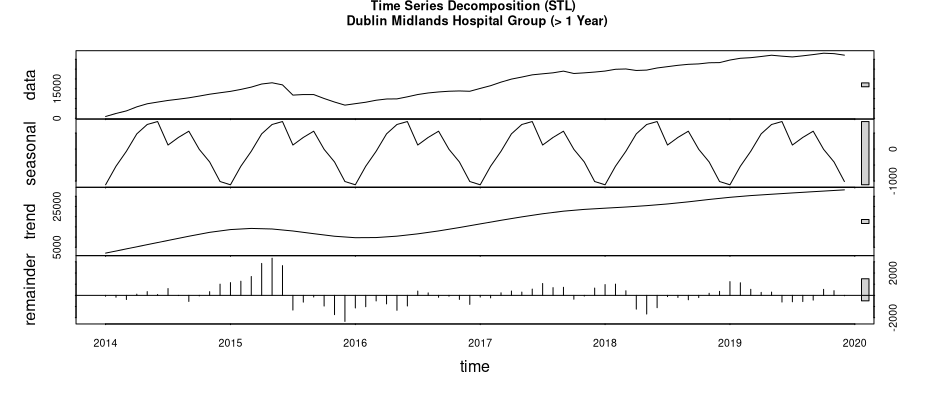
\includegraphics[width=0.7\linewidth]{/home/danny/MEGA/College/msc_data_analytics/data_science/ca3/hospital_waiting_lists/documentation/images/ts_dm_gt1yr} 

}

\caption{Time Series Decomposition - Dublin Midland Hospital Group patient numbers waiting more than a year.}\label{fig:ts-dm-gt1yr}
\end{figure}

\begin{figure}

{\centering 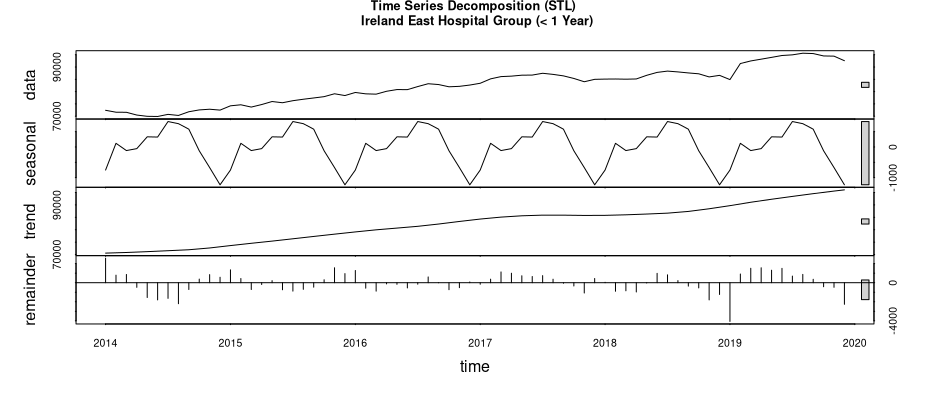
\includegraphics[width=0.7\linewidth]{/home/danny/MEGA/College/msc_data_analytics/data_science/ca3/hospital_waiting_lists/documentation/images/ts_ie_lt1yr} 

}

\caption{Time Series Decomposition - Ireland East Hospital Group patient numbers waiting less than a year.}\label{fig:ts-ie-lt1yr}
\end{figure}

\begin{figure}

{\centering 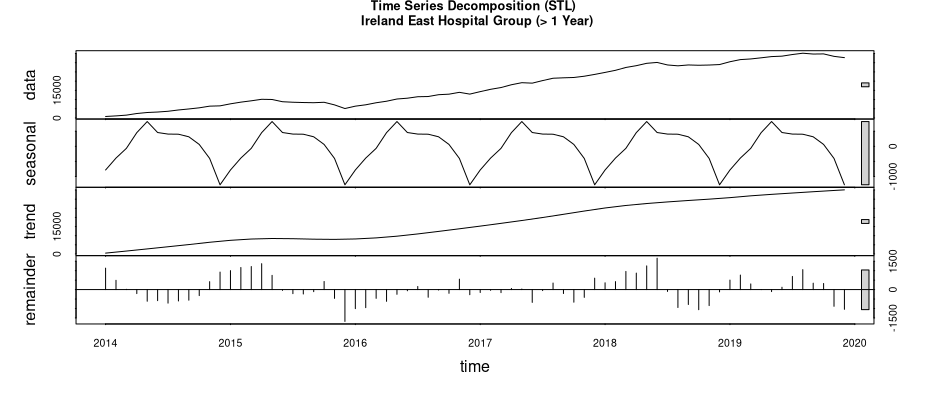
\includegraphics[width=0.7\linewidth]{/home/danny/MEGA/College/msc_data_analytics/data_science/ca3/hospital_waiting_lists/documentation/images/ts_ie_gt1yr} 

}

\caption{Time Series Decomposition - Ireland East Hospital Group patient numbers waiting more than a year.}\label{fig:ts-ie-gt1yr}
\end{figure}

\begin{figure}

{\centering 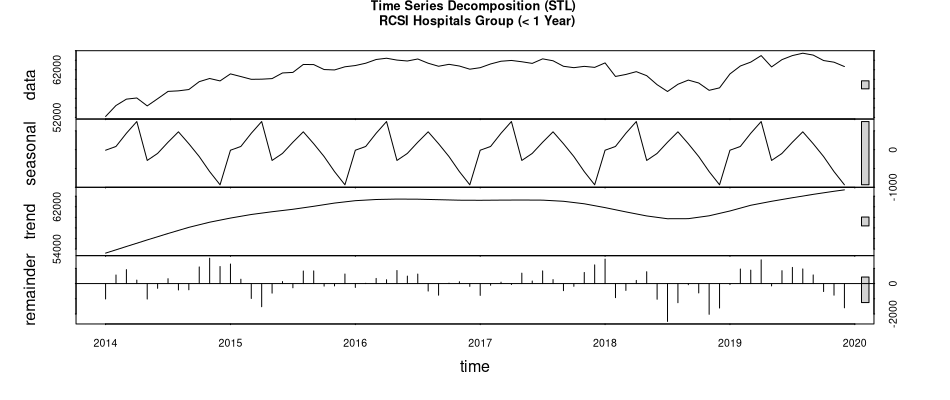
\includegraphics[width=0.7\linewidth]{/home/danny/MEGA/College/msc_data_analytics/data_science/ca3/hospital_waiting_lists/documentation/images/ts_rcsi_lt1yr} 

}

\caption{Time Series Decomposition - RCSI Hospitals Group patient numbers waiting less than a year.}\label{fig:ts-rcsi-lt1yr}
\end{figure}

\begin{figure}

{\centering 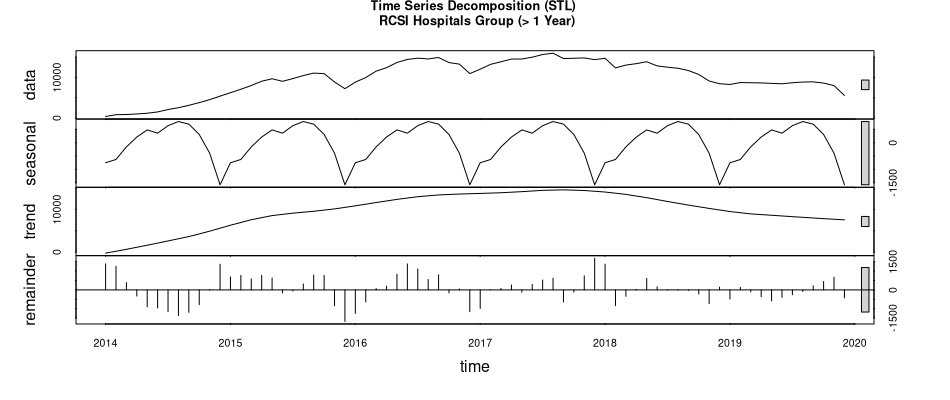
\includegraphics[width=0.7\linewidth]{/home/danny/MEGA/College/msc_data_analytics/data_science/ca3/hospital_waiting_lists/documentation/images/ts_rcsi_gt1yr} 

}

\caption{Time Series Decomposition - RCSI Hospitals Group patient numbers waiting more than a year.}\label{fig:ts-rcsi-gt1yr}
\end{figure}

\begin{figure}

{\centering 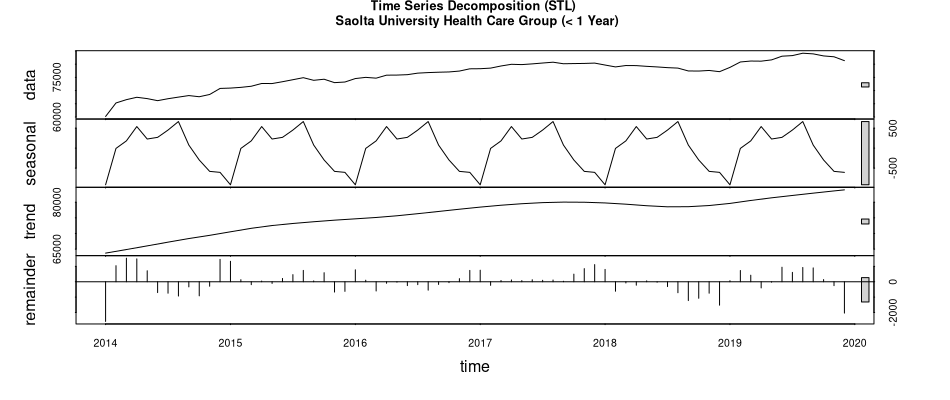
\includegraphics[width=0.7\linewidth]{/home/danny/MEGA/College/msc_data_analytics/data_science/ca3/hospital_waiting_lists/documentation/images/ts_saolta_lt1yr} 

}

\caption{Time Series Decomposition - Saolta University Health Care Group patient numbers waiting less than a year.}\label{fig:ts-saolta-lt1yr}
\end{figure}

\begin{figure}

{\centering 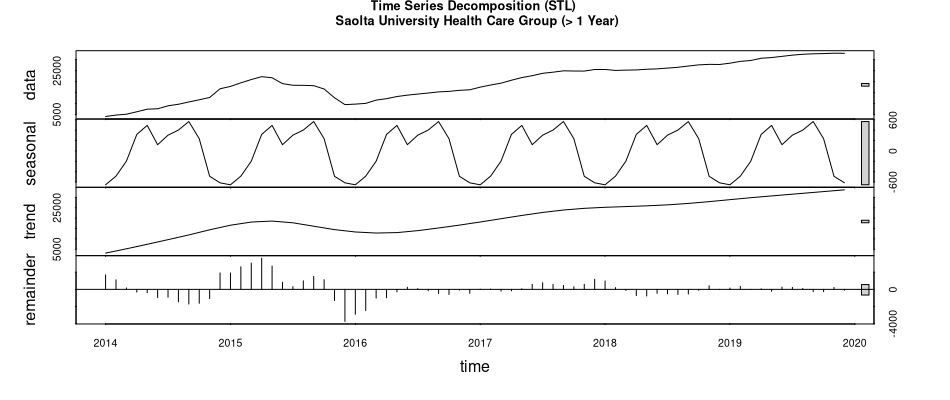
\includegraphics[width=0.7\linewidth]{/home/danny/MEGA/College/msc_data_analytics/data_science/ca3/hospital_waiting_lists/documentation/images/ts_saolta_gt1yr} 

}

\caption{Time Series Decomposition - Saolta University Health Care Group patient numbers waiting more than a year.}\label{fig:ts-saolta-gt1yr}
\end{figure}

\begin{figure}

{\centering 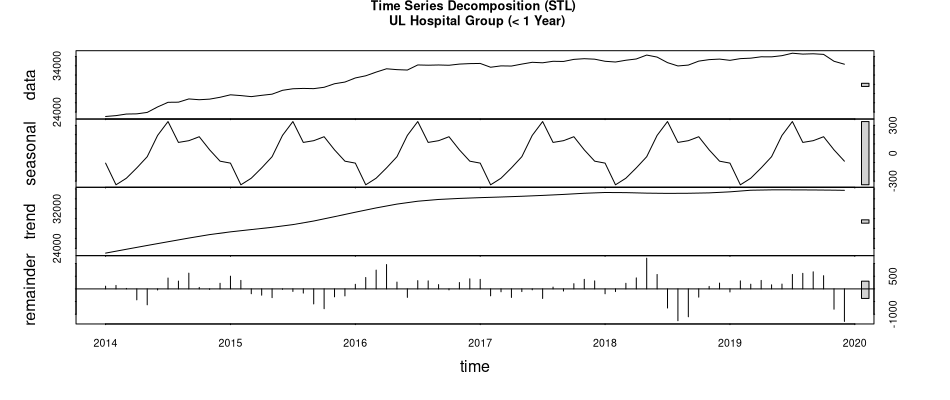
\includegraphics[width=0.7\linewidth]{/home/danny/MEGA/College/msc_data_analytics/data_science/ca3/hospital_waiting_lists/documentation/images/ts_ul_lt1yr} 

}

\caption{Time Series Decomposition - University of Limerick Hospital Group patient numbers waiting less than a year.}\label{fig:ts-ul-lt1yr}
\end{figure}

\begin{figure}

{\centering 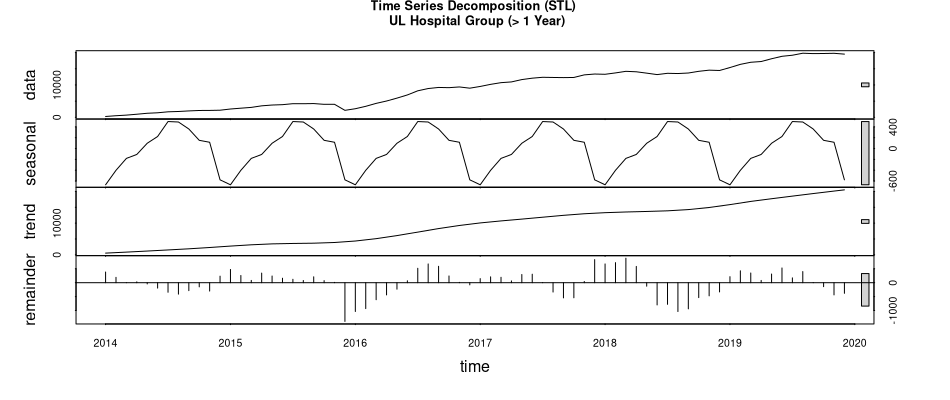
\includegraphics[width=0.7\linewidth]{/home/danny/MEGA/College/msc_data_analytics/data_science/ca3/hospital_waiting_lists/documentation/images/ts_ul_gt1yr} 

}

\caption{Time Series Decomposition - University of Limerick Hospital Group patient numbers waiting more than a year.}\label{fig:ts-ul-gt1yr}
\end{figure}

\begin{figure}

{\centering 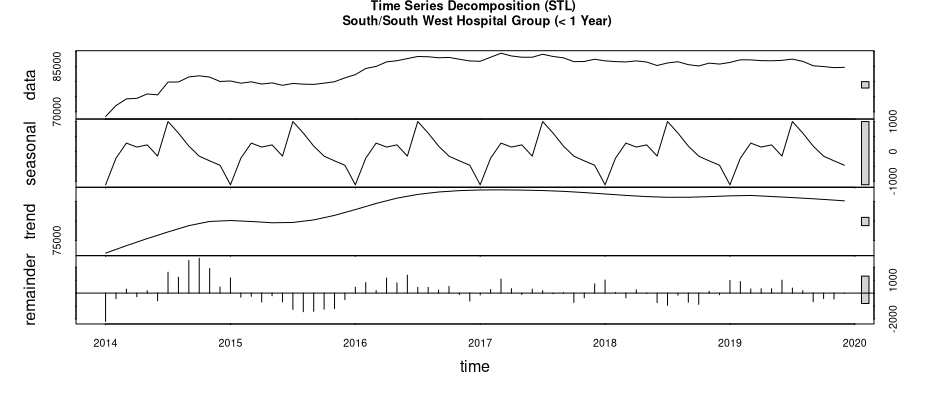
\includegraphics[width=0.7\linewidth]{/home/danny/MEGA/College/msc_data_analytics/data_science/ca3/hospital_waiting_lists/documentation/images/ts_ssw_lt1yr} 

}

\caption{Time Series Decomposition - South/South West Hospital Group patient numbers waiting less than a year.}\label{fig:ts-ssw-lt1yr}
\end{figure}

\begin{figure}

{\centering 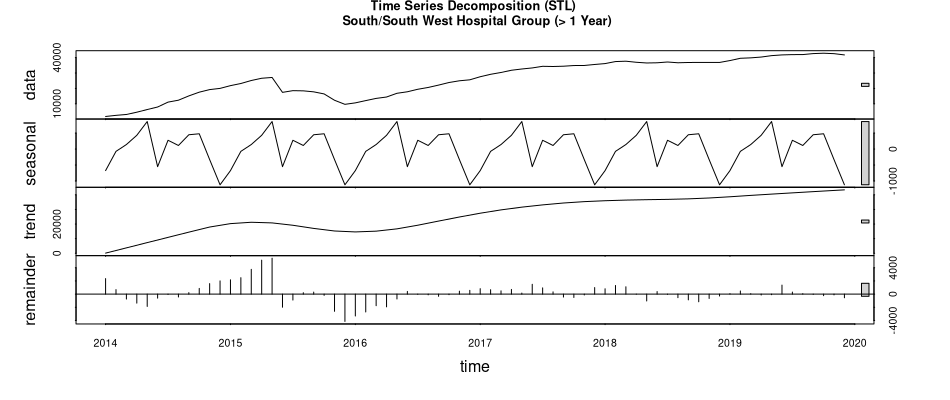
\includegraphics[width=0.7\linewidth]{/home/danny/MEGA/College/msc_data_analytics/data_science/ca3/hospital_waiting_lists/documentation/images/ts_ssw_gt1yr} 

}

\caption{Time Series Decomposition - South/South West Hospital Group patient numbers waiting more than a year.}\label{fig:ts-ssw-gt1yr}
\end{figure}

\end{document}
